\documentclass{article}
\usepackage{graphicx}
\title{Book note: Introduction To Bayesian Networks}
\date{20201006}

\begin{document}
\maketitle

\section{Ideas}

\begin{itemize}
    \item Is it possible to encapsulate dataset or expert knowledge into prior distribution
    to conduction ML, like perception tasks, in the bayesian way?
    \item Autonomous driving diagnose module (Bayesian implementation as expert system)
\end{itemize}

\section{Statement}

\begin{itemize}
    \item The multi-sensor fusion solution performs better than the single-sensor solution.
    From the aspect of information theory, it can be attributed to 
    the multi-sensor fusion solution has more observations, so that the entropy will be smaller and the uncertainty will get dropped.
\end{itemize}

\subsection{Relationship between joint entropy, conditional entropy and mutual information}
\begin{figure}[h]
\centering
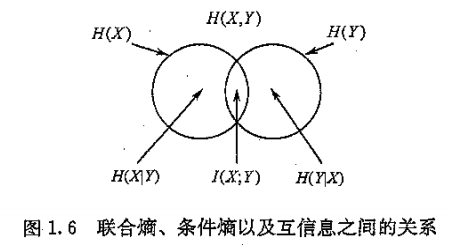
\includegraphics[width=0.6\columnwidth]{figs/relationship_entropy_mutualinfo.png}
\end{figure}

\subsection{Naive bayes model}
\begin{figure}[h]
\centering
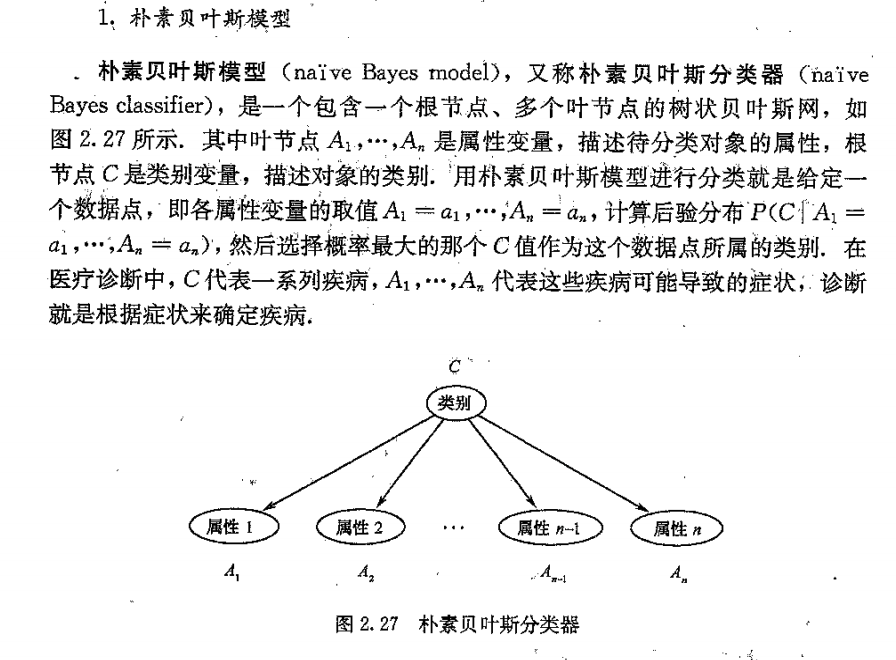
\includegraphics[width=1.05\columnwidth]{figs/naive_bayes.png}
\end{figure}

\subsection{MAP is NP-HARD}
\begin{figure}[h]
    \centering
    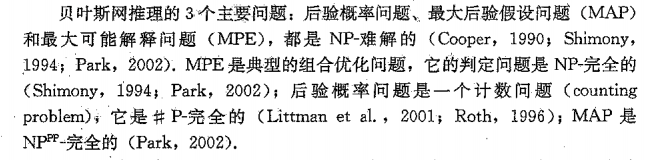
\includegraphics[width=1.05\columnwidth]{figs/nphard.png}
\end{figure}

\subsection{An MCMC example: Gibbs sampling}
\begin{figure}[h]
    \centering
    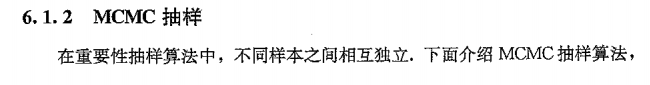
\includegraphics[width=1.05\columnwidth]{figs/mcmc1.png}
\end{figure}
\begin{figure}[h]
    \centering
    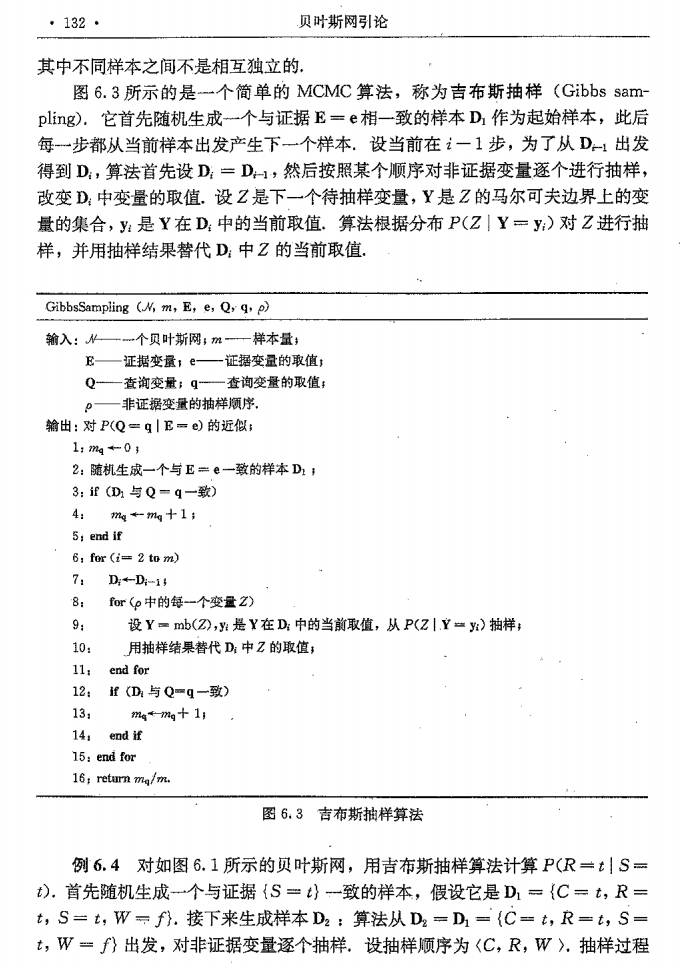
\includegraphics[width=1.05\columnwidth]{figs/mcmc2.png}
\end{figure}
\begin{figure}[h]
    \centering
    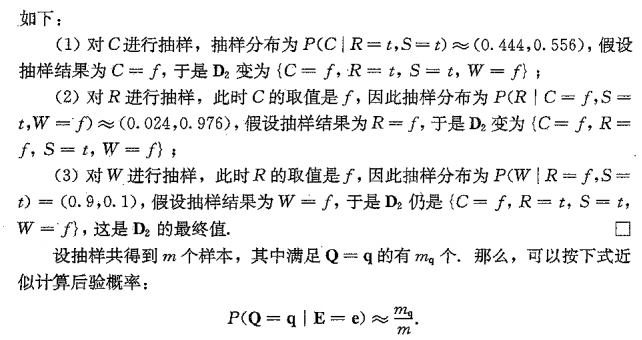
\includegraphics[width=1.05\columnwidth]{figs/mcmc3.png}
\end{figure}

\subsection{Why using Beta distribution instead of Gaussian as the prior distribution for MAP?}
It is because we want to use a prior distribution with a similar form as the likelihood.

\begin{figure}[h]
    \centering
    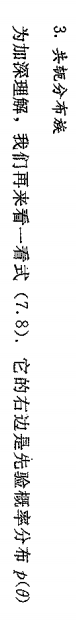
\includegraphics[width=1.05\columnwidth]{figs/conjugate_family1.png}
\end{figure}
\begin{figure}[h]
    \centering
    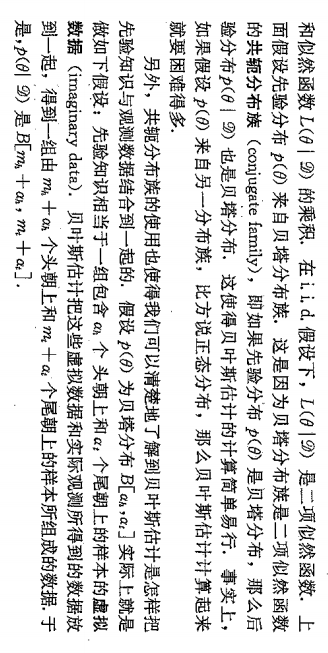
\includegraphics[width=1.05\columnwidth]{figs/conjugate_family2.png}
\end{figure}


\subsection{Property of MLE}
\begin{figure}[h]
    \centering
    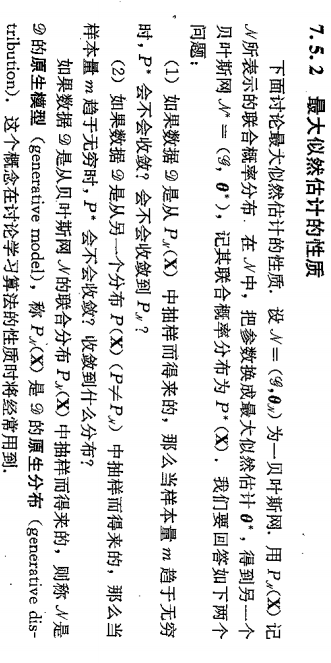
\includegraphics[width=1.05\columnwidth]{figs/mle_property.png}
\end{figure}

\section{Problems}
\begin{itemize}
    \item U-separation
    \item Latent variable analysis
\end{itemize}
\end{document}
